%%%%%%%%%%%%%%%%%%%%%%%%%%%%%%%%%%%%%%%%%
% Beamer Presentation
% Standard LaTeX Template used for creating presentation of Firebird-V Robot and other tutorials. 
% Author: Saurav Shandilya (e-Yantra Team)
% Reference: www.LaTeXTemplates.com Version 1.0 (10/11/12)
%
%%%%%%%%%%%%%%%%%%%%%%%%%%%%%%%%%%%%%%%%%

%----------------------------------------------------------------------------------------
%	PACKAGES AND THEMES
%----------------------------------------------------------------------------------------
		
\documentclass[table,10pt,red]{beamer}	% First line -- Define document class as Beamer which is used for creating presentation using Latex
\setbeamercolor{alerted text}{fg=blue} 	% Sets color of highlighted text during presentation.  
 

% The Beamer class comes with a number of default slide themes
% which change the colors and layouts of slides. Below this is a list
% of all the themes, uncomment each in turn to see what they look like.

%\usetheme{default}
%\usetheme{AnnArbor}
%\usetheme{Antibes}
%\usetheme{Bergen}
%\usetheme{Berkeley}
\usetheme{Berlin}		%used theme in present documents.
%\usetheme{Boadilla}
%\usetheme{CambridgeUS}
%\usetheme{Copenhagen}
%\usetheme{Darmstadt}
%\usetheme{Dresden}
%\usetheme{Frankfurt}
%\usetheme{Goettingen}
%\usetheme{Hannover}
%\usetheme{Ilmenau}
%\usetheme{JuanLesPins}
%\usetheme{Luebeck}
%\usetheme{Madrid}
%\usetheme{Malmoe}
%\usetheme{Marburg}
%\usetheme{Montpellier}
%\usetheme{PaloAlto}
%\usetheme{Pittsburgh}
%\usetheme{Rochester}
%\usetheme{Singapore}
%\usetheme{Szeged}
%\usetheme{Warsaw}

% As well as themes, the Beamer class has a number of color themes
% for any slide theme. Uncomment each of these in turn to see how it
% changes the colors of your current slide theme.

%\usecolortheme{albatross}
%\usecolortheme{beaver}
%\usecolortheme{beetle}
%\usecolortheme{crane}
%\usecolortheme{dolphin}
%\usecolortheme{dove}
%\usecolortheme{fly}
%\usecolortheme{lily}
%\usecolortheme{orchid}
%\usecolortheme{rose}
%\usecolortheme{seagull}
%\usecolortheme{seahorse}
%\usecolortheme{whale}
%\usecolortheme{wolverine}

%\setbeamertemplate{footline} % To remove the footer line in all slides uncomment this line
%\setbeamertemplate{footline}[page number] % To replace the footer line in all slides with a simple slide count uncomment this line

%\setbeamertemplate{navigation symbols}{} % To remove the navigation symbols from the bottom of all slides uncomment this line
%}

%------------------------------------------------------------------------------------------
%	\usepackage is required for including various features like images, table, references etc.
%	Packages must be installed before using. These can be istalled through package manager. 
%   Various packages have dependencies and for using such packages all dependent packages must be used. 
%-----------------------------------------------------------------------------------------
\usepackage{beamerthemeshadow} % theme shadow for visual 
\usepackage{beamerthemesplit} % Creates minipage (for showing multiple images and text) on same page  
\usepackage{graphicx} % Allows including images
\usepackage{booktabs} % Allows the use of \toprule, \midrule and \bottomrule in tables
\usepackage{xcolor}
\usepackage{booktabs,array}
\usepackage{listings}
\usepackage{hyperref}	% Required for including hyperlink in document
\usepackage{verbatim,moreverb} % Required for including code snippet.
\usepackage{colortbl}
\usepackage{multirow}	% Required for creating multiple row tables
\usepackage{tikz}		% Required for drawing shapes such as circles, arrowed line, etc. 
\usetikzlibrary{arrows}

% logo
\logo{
\includegraphics[height=1cm]{iitblogo.pdf}} % includes logo at bottom of all slides 

%----------------------------------------------------------------------------------------
%	TITLE PAGE
%----------------------------------------------------------------------------------------
% sf family, bold font
\sffamily \bfseries
% content inside [] appears at bottom of all page. content inside {} appears on first page as title. double backslash means line change 
\title
[
	Firebird ATmega2560 Robotics Research Platform	% bottom of all page
	\hspace{0.5cm}
	\insertframenumber/\inserttotalframenumber
]
{
	Serial Communication On Firebird V Robot
}

\author
[
	www.e-yantra.org 	%Name at bottom of all page 
]
% author name on title slide
{
	e-Yantra Team \\
  Embedded Real-Time Systems Lab\\
  Indian Institute of Technology-Bombay \\
}
\date
{
IIT Bombay \\ {\today}	%\today picks system date on title slide
}

\begin{document} % IN LATEX ALL DOCUMENT/REPORT/PRESENTATION STARTS WITH \begin{document} AND ENDS WITH \end{document}

\begin{frame}	% FRAME MEANS SLIDE. \begin{frame} STARTS THE SLIDE AND \end{frame} ENDS THE SLIDE
	\titlepage % Print the title page as the first slide
\end{frame}
\section*{Outline}
% START OF SECOND SLIDE
\begin{frame}
	\frametitle{Agenda for Discussion} % Table of contents slide, comment this block out to remove it
	\tableofcontents % Throughout your presentation, if you choose to use \section{} and \subsection{} commands, these will automatically be printed on this slide as an overview of your presentation
\end{frame}
%----------------------------------------------------------------------------------------
%	PRESENTATION SLIDES
%----------------------------------------------------------------------------------------

%------------------------------------------------
\section{Introduction to Serial Communication} % Sections can be created in order to organize your presentation into discrete blocks, all sections and subsections are automatically printed in the table of contents as an overview of the talk
%------------------------------------------------

\subsection{What is Serial Communication} % A subsection can be created just before a set of slides with a common theme to further break down your presentation into chunks

% Start of Third slide
\begin{frame}
	\frametitle{What is Serial Communication}
 	\color{red}Serial communication\color{black} \  is the process of sending data one bit at a time, sequentially, over a communication channel. This is in contrast to parallel communication, where several bits are sent as a whole, on a link with several parallel channels. \\
 		
 		
\end{frame}

%------------------------------------------------

\subsection{Needs and Ways of Serial Communication} % A subsection can be created just before a set of slides with a common theme to further break down your presentation into chunks

% Start of Fourth slide
\begin{frame}[shrink]
	\frametitle{Needs and Ways of Serial Communication}
	\textbf{Needs of Serial Communication.} 	
 	\begin{itemize}  % Shows text in bullet point 		
		\item <+-|alert@+> To establish a communication between devices like PCs, Tablets and other external devices.
		\item <+-|alert@+> To establish communication between 
			\begin{enumerate}
				\item <+-|alert@+> Two/multiple robots
				\item <+-|alert@+> Robots and external devices
			\end{enumerate}
	\end{itemize}
 		
	\textbf{Ways of Serial Communication} 	
 	\begin{itemize}  % Shows text in bullet point 			
		\pause		
		\item Wired communication
			\begin{enumerate}
				\item <+-|alert@+> USB
				\item <+-|alert@+> RS232
				\item <+-|alert@+> etc.
			\end{enumerate}
		\item Wireless communication
			\begin{enumerate}
				\item <+-|alert@+> Zigbee
				\item <+-|alert@+> Bluetooth
				\item <+-|alert@+> WiFi
				\item <+-|alert@+> etc.				
			\end{enumerate}
	\end{itemize} 		
 		
 		
\end{frame}

%------------------------------------------------
% Start of fifth slide
\subsection{Inbuilt UART pins of ATmega 2560} % A subsection can be created just before a set of slides with a common theme to further break down your presentation into chunks
\begin{frame}
\frametitle{Inbuilt UART pins of ATmega 2560}
ATmega 2560 supports 4 UARTs(UART 0-3). In Firebird V these are configured to  following devices by default.
	\begin{itemize}
		\item <+-|alert@+> UART0 to  Zigbee Wireless module
		\item <+-|alert@+> UART1 to  RS232 Serial port
		\item <+-|alert@+> UART2 to  FT232 USB serial converter
		\item <+-|alert@+> UART3 to  expansion port
	\end{itemize}

\pause
\begin{table}
\begin{tabular}{c c c c}
\toprule
\textbf{UARTx} & \textbf{Rx} & \textbf{Tx} & \textbf{module} \\
\midrule
UART0 & PORTE0 & PORTE1 & Zigbee\\
UART1 & PORTD2 & PORTD3 & RS232\\
UART2 & PORTH0 & PORTH1 & USB\\
UART3 & PORTJ0 & PORTJ1 & expansion slot\\
\bottomrule
\end{tabular}
\end{table}
\end{frame}
%----------------------------------------------
%------------------------------------------------
% Start of sixth slide
\section{Registers used in serial communication}
\subsection{Types of registers}
\begin{frame}
\frametitle{Types of Registers}
\textbf{These are the various registers involved in serial communication :}
	\begin{itemize}
		\item <+-|alert@+> UCSRnA = USART control and status register nA.
		\item <+-|alert@+> UCSRnB = USART control and status register nB.
		\item <+-|alert@+> UCSRnC = USART control and status register nC.
		\item <+-|alert@+> UBRRnL \& UBRRnH = USART baud rate registers.
		\item <+-|alert@+> UDRn = USART input/output register n.
	\end{itemize}
	\begin{small}Note: n represents the UART number which can be 0,1,2,3....\end{small}
\end{frame}
%------------------------------------------------
% Start of seventh slide
\subsection{UCSRnA}
	\begin{frame}
	\frametitle{UCSRnA-Control and Status Register nA.}
		\begin{table}
		\begin{tabular}{!{\vrule width 0.8pt}>{\columncolor[gray]{0.9}[0.8\tabcolsep]}c|>{\columncolor[gray]{0.9}[0.8\tabcolsep]}c|>{\columncolor[gray]{0.9}[0.8\tabcolsep]}l|>{\columncolor[gray]{0.9}[0.8\tabcolsep]}c!{\vrule width 0.8pt}}
		\toprule
		\textbf{Bit} & \textbf{Symbol} & \textbf{Description} & \textbf{Bit Value} \\
		\midrule
		\pause
		\vspace{2pt}
			7 & RxCn & Receive Complete & 0\\
			\pause
			\vspace{2pt}
			6 & TxCn & Transmit Complete & 0\\
			\pause
			\vspace{2pt}
			5 & UDREn & Data Register Empty & 0\\
			\pause
			\vspace{2pt}
			4 & FEn & Frame Error & 0\\
			\pause
			\vspace{2pt}
			3 & DORn & Data Over-Run & 0\\
			\pause
			\vspace{2pt}
			2 & UPEn & Parity Error & 0\\
			\pause
			\vspace{2pt}
			1 & U2Xn & Double transmission speed & 0\\
			\pause
			\vspace{2pt}
			0 & MPCMn & MultiProcessor Communication Mode & 0\\
		
		\bottomrule
		\end{tabular}
		\end{table}
		\pause		
		\begin{Large}
			\begin{flushright}							
				UCSRnA=0x00\hspace*{10mm}
			\end{flushright}
		\end{Large}
	\end{frame}
	
%------------------------------------------------
% Start of eigth slide
\subsection{UCSRnB}
	\begin{frame}
	\frametitle{UCSRnB-Control and Status Register nB.}
		\begin{table}
		\begin{tabular}{!{\vrule width 0.8pt}>{\columncolor[gray]{0.9}[0.8\tabcolsep]}c|>{\columncolor[gray]{0.9}[0.8\tabcolsep]}c|>{\columncolor[gray]{0.9}[0.8\tabcolsep]}l|>{\columncolor[gray]{0.9}[0.8\tabcolsep]}c!{\vrule width 0.8pt}}
		\toprule
		\textbf{Bit} & \textbf{Symbol} & \textbf{Description} & \textbf{Bit Value} \\
		\midrule
		\pause
		\vspace{2pt}
			7 & RxCIEn & Receive Complete Interrupt Enable & 1\\
			\pause
			\vspace{2pt}			
			6 & TxCIEn & Transmit Complete Interrupt Enable & 0\\
			\pause
			\vspace{2pt}			
			5 & UDRIEn & Data Register Empty & 0\\
			\pause
			\vspace{2pt}			
			4 & RXENn & Receiver Enable & 1\\
			\pause
			\vspace{2pt}			
			3 & TXENn & Transmiter Enable & 1\\
			\pause
			\vspace{2pt}		
			2 & UCSZn2 & char size n & 0\\
			\pause
			\vspace{2pt}			
			1 & RXB8n & Receive data bit 8 & 0\\
			\pause
			\vspace{2pt}			
			0 & TXB8n & Transmit data bit 8 & 0\\
		
		\bottomrule
		\end{tabular}
		\end{table}
		\pause		
		\begin{Large}
			\begin{flushright}				
				UCSRnB=0x98\hspace*{10mm}
			\end{flushright}
		\end{Large}
	\end{frame}	
	
	
	
	
%------------------------------------------------
% Start of ninth slide
\subsection{UCSRnC}
	\begin{frame}
	\frametitle{UCSRnC-Control and Status Register nC.}
		\begin{table}
		\begin{tabular}{!{\vrule width 0.8pt}>{\columncolor[gray]{0.9}[0.8\tabcolsep]}c|>{\columncolor[gray]{0.9}[0.8\tabcolsep]}c|>{\columncolor[gray]{0.9}[0.8\tabcolsep]}l|>{\columncolor[gray]{0.9}[0.8\tabcolsep]}c!{\vrule width 0.8pt}}
		\toprule
		\textbf{Bit} & \textbf{Symbol} & \textbf{Description} & \textbf{Bit Value} \\
		\midrule
		\pause
		\vspace{2pt}
			7 & UMSELn1 & USART Mode Select & 0\\
			6 & UMSELn0 & USART Mode Select & 0\\
			\pause
			\vspace{2pt}			
			5 & UPMn1 & Parity Mode & 0\\
			4 & UPMn0 & Parity Mode & 0\\
			\pause
			\vspace{2pt}			
			3 & USBSn & Stop Bit Select & 0\\
			\pause
			\vspace{2pt}			
			2 & UCSZn1 & Character Size & 1\\
			1 & UCSZn0 & Character Size & 1\\
			\pause
			\vspace{2pt}			
			0 & UCP0Ln & Clock polarity & 0\\
		
		\bottomrule
		\end{tabular}
		\end{table}
		\pause		
		\begin{Large}
			\begin{flushright}
				UCSRnC=0x06\hspace*{10mm}
			\end{flushright}
		\end{Large}
	\end{frame}	
	
	

%------------------------------------------------
% Start of tenth slide
\begin{frame}[shrink]

\begin{figure}
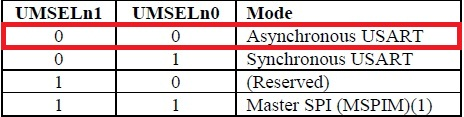
\includegraphics[width=0.8\linewidth]{UMSE}
\end{figure}
\pause
\begin{figure}
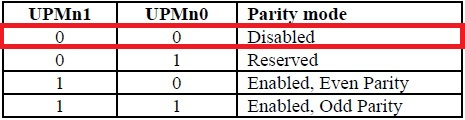
\includegraphics[width=0.8\linewidth]{parity}
\end{figure}
\pause
\begin{figure}
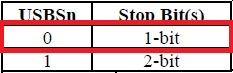
\includegraphics[width=0.4\linewidth]{stop_bit}
\end{figure}
\pause
\begin{figure}
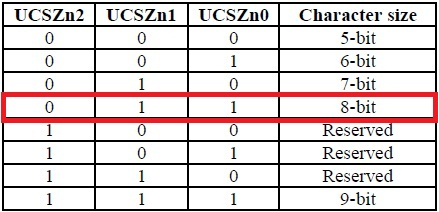
\includegraphics[width=0.8\linewidth]{bit}
\end{figure}
\end{frame}	
	%------------------------------------------------
% Start of eleventh slide
\subsection{UBRRnL \& UBRRnH}
	\begin{frame}[shrink]
	\frametitle{UBRRnL \& UBRRnH-Baud Rate Registers}
	\begin{Large}These two registers are used to set baud rates.\\ Crystal frequency is 14.7456MHz.\end{Large}	
	\pause	\\
	\begin{block}{\textbf{example:}}
			
		 Let us consider for a baud rate of 9600 \\
		 $$UBRR=\left\{\frac{System clock}{16*Baud Rate}\right\}-1$$		
		 $$UBRR=\left\{\frac{14.7456Mhz}{16*9600}\right\}-1$$
		 $$UBRR=95$$
		 $$UBRR=0x5FH$$
		 $$UBRRH=0x00H$$
		 $$UBRRL=0x5FH$$		
	\end{block}
	\begin{Large}Note:While loading values in UBRR register load values in the UBRRH register first.\end{Large}
				
	\end{frame}
	
	%------------------------------------------------
% Start of twelveth slide
\subsection{UDRn}
	\begin{frame}
	\frametitle{UDRn-USART I/O Data Register n}
	\begin{itemize}
		\item <+-|alert@+> The USART Transmit Data Buffer Register and USART receive data buffer register share the same I/O address referred to as USART data Registers or UDR.
		\item <+-|alert@+> The transmit Data Buffer register(TxB) will be the destination for data written to the UDRn register location.
		\item <+-|alert@+> Reading the UDRn Register location will return the contents of the received data buffer register(RxB).
	\end{itemize}
	\end{frame}


	%------------------------------------------------
% Start of thirteenth slide
\section{Interrupts in Serial communication}
\subsection{Receive Complete ISR}
\begin{frame}
	\frametitle{Receive Complete ISR}	
	\begin{block}{Receive Complete ISR}
		SIGNAL(SIG\_USARTn\_RECV)\color{red}  // ISR for receive complete interrupt.\color{black}\\
		\{ \\
		\ \ \ 	data = UDRn; \color{red}      //Making a copy of data from UDRn in 'data' variable.\color{black} \\
		\}
	\end{block}
		If RXCIE interrupt is enabled then receive complete interrupt triggers ISR.
\end{frame}

	%------------------------------------------------
% Start of fourteenth slide

	\subsection{Data Register empty ISR}	
	\begin{frame}	
	\frametitle{Data Register empty ISR}
	\begin{block}{Data Register empty ISR}
		SIGNAL(SIG\_USARTn\_DATA) \color{red} // ISR for Data Register empty interrupt.\color{black}\\
		\{ \\
		\ \ \ 	UDRn = tx\_data; \color{red}      //data that need to be transmitted is transferred to\\ \hspace{50mm} UDRn\color{black}\\
		\}
	\end{block}
		If UDRIE interrupt is enabled then UDRn data register empty interrupt triggers ISR. This ISR then loads next data byte to be transmitted into UDRn.

	\end{frame}

	%------------------------------------------------
% Start of fifteenth slide

	\subsection{Transmit Complete ISR}
	\begin{frame}
	\frametitle{Transmit Complete ISR}	
	\begin{block}{Transmit Complete ISR}
		SIGNAL(SIG\_USARTn\_TRANS)\color{red}  // ISR for Transmit complete interrupt.\color{black}\\
		\{ \\
			\color{red}	//Insert your code\color{black}\\
		\}
	\end{block}
		If TXCIE interrupt is enabled then transmit complete interrupt triggers ISR.
	\end{frame}
	
\section{C Code}
%------------------------------------------------
% Start of sixteenth slide
\subsection{UART initialization}
	\begin{frame}
	\pause
		\begin{block}{UART initialization}
			\color{red} //Function To Initialize UART1
\\			// desired baud rate=9600
\\			// actual baud rate=9600 (error 0.0%)
\\			// char size=8 bit
\\			// parity=Disabled
\\			// stop bit=1 \color{black}
\\			void uart0\_init(void)
\\			\{
\\			\ \ 	 UCSRB = 0x00;\color{red} //disable while setting baud rate\color{black}
\\			\ \ 	 UCSRA = 0x00;
\\			\ \ 	 UCSRC = 0x86;
\\			\ \ 	 UBRRL = 0x2F;\color{red} //set baud rate lo  \color{black}
\\			\ \ 	 UBRRH = 0x00;\color{red} //set baud rate hi\color{black}
\\			\ \ 	 UCSRB = 0x98; 
\\			\}
		\end{block}
	\end{frame}
	
	
%\section*{Demonstration and Thank You}
%------------------------------------------------
% Start of seventeenth slide
%\subsection*{Demonstration}
\begin{frame}
	\begin{huge}
		\color{red}
			\hskip4cm
				\begin{center}				
					\textit{\Huge Demonstration} \\[50pt]
				\end{center}
			\hskip3cm
		\color{black}
	\end{huge}
\end{frame}
%------------------------------------------------
% Start of eightteenth slide
%\subsection*{Thank You} % A subsection can be created just before a set of slides with a common theme to further break down your presentation into chunks
\begin{frame}
\hskip4cm
\textbf{\LARGE Thank You!} \\[20pt]
\hskip3cm
\scriptsize Post your queries on: 
\hyperref[helpdesk@e-yantra.org]{\color{blue} helpdesk@e-yantra.org \color{black}} 
\end{frame}
%----------------------------------------------------------------------------------------



	
	
\end{document} 